\documentclass[12pt]{article}
\usepackage[margin=1in]{geometry}
\usepackage{times}
\usepackage{parskip}
\usepackage{titlesec}
\usepackage{graphicx}
\usepackage{float}
\usepackage{hyperref}
\usepackage{cite}
\usepackage{amsmath}
\usepackage{tikz}
\usetikzlibrary{shapes.geometric, arrows.meta, positioning, calc}

% ---- Section formatting ----
\titleformat{\section}{\large\bfseries}{{\thesection.}}{0.5em}{}
\titleformat{\subsection}{\normalsize\bfseries}{{\thesubsection}}{0.5em}{}
\titleformat{\subsubsection}{\normalsize\bfseries}{{\thesubsubsection}}{0.5em}{}

\begin{document}

% ========== Title Page ==========
\begin{center}
\vspace*{2cm}
{\LARGE \textbf{ButterFlight}}\\[0.4cm]
{\large Maya Plug-in Design Document}\\[3cm]
{\large By: Cecilia Chen and Yiding Tian}\\[4cm]
{\large Based on:}\\[0.3cm]
{\normalsize A Practical Model for Realistic Butterfly Flight Simulation.}\\[0.2cm]
{\normalsize Chen, Q., Lu, T., Tong, Y., Luo, G., Jin, X., and Deng, Z., 2022.}\\
{\normalsize ACM Transactions on Graphics (TOG).}\\[3cm]
{\large CIS 6600 --- Advanced Topics in Computer Graphics and Animation}\\[0.3cm]
{\large Instructor: Dr.~Stephen Lane}
\end{center}

\newpage

% ========== Project Summary ==========
\section*{Project Summary}

Realistic butterfly flight animation is a recurring need in film, games, and virtual
environments, yet no dedicated authoring tool exists for it. Hand-keying the erratic,
noisy trajectories characteristic of real butterfly flight is prohibitively tedious,
and CFD-based simulation is far too slow for production use---leaving artists with
crude approximations that break the illusion of life.

ButterFlight addresses this gap by providing a Maya plug-in that generates physically
plausible butterfly flight animations through a force-based simulation model. The
design goals are to faithfully reproduce the characteristic features of real butterfly
flight---including wing-abdomen coupling, aerodynamic lift and drag, and inherent
trajectory noise---while keeping the interface simple enough for a generalist animator
to use without any background in aerodynamics or simulation.

The primary target audience is VFX artists and technical directors working in film,
games, or real-time virtual environments who need to populate a scene with one or more
butterflies without spending hours on hand animation. Users are expected to have
basic Maya modeling and rigging knowledge but require no knowledge of the underlying
physics.

ButterFlight exposes a MEL-scripted UI panel from which the user can load a rigged
butterfly mesh, set simulation parameters (flapping frequency, amplitude, wind
direction and strength, swarm size), optionally attach the butterfly to a path curve,
and bake the resulting motion as keyframed skeletal animation. Supported output modes
include single-butterfly free flight, path following, wind interaction, and swarm
aggregation. The final animation can be exported via Alembic or FBX for use in any
downstream pipeline.

The core simulation is implemented as a Maya C++ plug-in (\texttt{.mll}) built against
the Maya 2026 API. It runs the three-module algorithm from Chen et al.\ 2022:
parametric maneuvering functions with wing-abdomen interaction, a force model combining
quasi-steady aerodynamic forces with a curl-noise vortex force, and a maneuvering
controller that decouples body translation from posture adjustment. The UI and scene
setup utilities are written in MEL/Python.

The development schedule targets an alpha version (single-butterfly simulation with
basic aerodynamic forces and MEL UI) by March 25th, a beta version (full force model,
path following, and swarm support) by April 15th, and a final polished version
with tutorials and demo scenes due May 11th.

\newpage

% ========== Section 1: Authoring Tool Design ==========
\section{Authoring Tool Design}

\subsection{Significance of Problem or Production/Development Need}

Butterflies appear in a wide range of production contexts---background ambience in
nature documentaries, hero insect shots in animated features, environmental
atmosphere in video games and virtual reality, and educational simulations.
Despite this demand, no dedicated authoring tool for butterfly flight animation
exists in any major DCC package. Artists currently resort to one of three
unsatisfactory options: (1)~hand-keying every frame of wing and body motion,
which is extremely time-consuming given the high flapping frequency
($\approx$9--11~Hz) and the erratic, noisy trajectories that characterize real
butterfly flight; (2)~looping a pre-made cycle animation, which produces
robotic, repetitive motion with no dynamic response to the environment; or
(3)~outsourcing to a CFD-based simulation, which requires specialist knowledge,
days of computation time, and produces results that are difficult to art-direct.

The fundamental challenge is that butterfly flight is governed by closely coupled
wing-body interaction: the abdomen oscillates in counterphase to the wings,
the thorax pitches with each stroke, and an inherent vortex-driven noise keeps
the trajectory unpredictable. Without capturing all three effects simultaneously
it is impossible to produce convincing butterfly animation in any setting, whether
for a single hero butterfly or a swarm of hundreds. A tool that automates this
physics while remaining controllable and fast enough for interactive use in Maya
would directly address this production gap.

\subsection{Technology}

ButterFlight is based on the 2022 ACM SIGGRAPH paper \textit{``A Practical Model
for Realistic Butterfly Flight Simulation''} by Qiang Chen, Tingsong Lu, Yang
Tong, Guoliang Luo, Xiaogang Jin, and Zhigang Deng. The paper proposes the first
force-based model specifically designed for real-time butterfly flight simulation
in graphics and animation applications. The approach is organized into three
inter-connected modules, as illustrated in Figure~\ref{fig:overview}.

\begin{figure}[H]
  \centering
  \includegraphics[width=0.85\textwidth]{img/overview_figure.png}
  \caption{Pipeline overview of the Chen et al.\ 2022 approach. Starting from a rigged
    butterfly mesh, the system computes aerodynamic and vortex forces, then applies a
    maneuvering controller to generate body motion and trajectories
    (reproduced from Chen et al.\ 2022, Fig.~1).}
  \label{fig:overview}
\end{figure}

The first module, \textbf{butterfly modeling}, represents the butterfly as a
hierarchical skeleton (thorax as root, four wings, abdomen) driven by parametric
maneuvering functions. Five joint angles---thorax pitch $\theta_\beta$, fore-wing
flap $\theta_\gamma$, fore-wing feather $\theta_\zeta$, fore-wing sweep
$\theta_\psi$, and abdomen rotation $\theta_\phi$---are computed each frame via a
cosine-based periodic function (Equation~1 of the paper) whose amplitude and
frequency scale with the butterfly's current velocity. The abdomen is assigned a
phase offset of $-180^\circ$ relative to the wings to reproduce the
counterphase oscillation observed in real Monarch butterflies~\cite{Sridhar2016}.
Figure~\ref{fig:model} illustrates the five joint angles and their geometric definitions.

\begin{figure}[H]
  \centering
  \includegraphics[width=0.8\textwidth]{img/model_figure.png}
  \caption{Joint angle definitions of the butterfly skeleton model.
    The thorax pitch angle $\theta_\beta$ and abdomen rotation $\theta_\phi$ are shown
    in (d) and (b); the fore-wing flap angle $\theta_\gamma$ and feather angle
    $\theta_\zeta$ are shown in (a); the sweep angle $\theta_\psi$ is shown in (c)
    (reproduced from Chen et al.\ 2022, Fig.~4).}
  \label{fig:model}
\end{figure}

The second module, \textbf{forces computation}, computes two forces acting on the
butterfly at each time step. A simplified aerodynamic force (lift and drag per
wing polygon, Equations~4--6) is derived from the quasi-steady theory of
Ellington~(1984), using empirical lift and drag coefficient polynomials as a
function of the local angle of attack. A vortex force (Equation~7) is computed
from a curl-noise field~\cite{Bridson2007} seeded with Perlin noise~\cite{Perlin2002}
and applied to the thorax centre of mass, simulating the wake of the flapping
wings and producing the inherent chaotic trajectory noise characteristic of
real butterfly flight.

The third module, \textbf{maneuvering control}, decouples body translation from
body posture. At each time step the composite force (aerodynamic + vortex +
gravity + optional attraction toward a target or path keypoint) is integrated
via Newton's second law to obtain velocity. Wing frequency and amplitude are
then updated using a sliding-window smoother (Equation~12) to avoid abrupt
changes across flapping cycles. Figure~\ref{fig:maneuver} shows the phase
relationships of the five joint angles across one full flapping cycle.

\begin{figure}[H]
  \centering
  \includegraphics[width=0.82\textwidth]{img/manuever_figure.png}
  \caption{Phase shifts of all five maneuvering angles during one wing-flapping cycle
    (downstroke $t_0$ to upstroke $t_1$). The abdomen angle $\theta_\phi$ is driven
    at $-180^\circ$ phase offset relative to the flap angle $\theta_\gamma$,
    reproducing counterphase oscillation
    (reproduced from Chen et al.\ 2022, Fig.~5).}
  \label{fig:maneuver}
\end{figure}

We chose this paper because it is the only published method that addresses all
three distinguishing features of butterfly flight (wing-abdomen coupling,
aerodynamic force, and inherent trajectory noise) in a single, real-time
capable framework. The algorithm is self-contained, mathematically explicit,
and maps cleanly onto Maya's joint/keyframe animation system, making it an
ideal candidate for implementation as an interactive authoring tool. The paper
also includes quantitative parameter tables (Tables~2 and~3) for two butterfly
species, providing concrete values to initialize our simulation.

\subsection{Design Goals}

ButterFlight addresses the production need by providing a Maya plug-in that
automates the entire butterfly flight simulation pipeline---from joint-angle
computation through trajectory integration to keyframe baking---behind a
single, artist-friendly UI panel. The animator supplies a rigged butterfly
mesh and a handful of high-level parameters; the plug-in handles all
physics. The resulting output is standard Maya keyframe animation that can be
refined by hand, cached to Alembic, or exported to any downstream pipeline
without any dependency on the plug-in at render time.

\subsubsection{Target Audience}

The primary users of ButterFlight are \textbf{VFX artists and technical directors}
in film, television, game development, and real-time virtual production who need
to include one or more butterflies in a scene. This includes generalist
animators who want a quick, convincing butterfly without manual keyframing, and
TDs who need to populate a background environment with a swarm of butterflies in
an automated, art-directable way. Secondary users are students and researchers
who wish to explore physically-based insect animation.

Users are expected to have basic Maya literacy---they should know how to import
meshes, work with joints and skinning, and use basic curve tools for path
creation. No background in aerodynamics, physics simulation, or programming is
required to operate the tool.

\subsubsection{User Goals and Objectives}

With ButterFlight, a user should be able to accomplish the following:

\begin{itemize}
  \item \textbf{Single butterfly, free flight.} Simulate one butterfly flying
    with inherently noisy, physically plausible motion without specifying any
    path, suitable for ambient background use.

  \item \textbf{Single butterfly, path following.} Attach the simulation to a
    user-drawn NURBS curve so the butterfly broadly follows an art-directed
    trajectory while still exhibiting natural erratic deviations and wing-body
    dynamics.

  \item \textbf{Wind interaction.} Apply a constant or time-varying wind vector
    to the simulation and observe the butterfly attempt to recover stable flight,
    producing realistic spiraling responses.

  \item \textbf{Swarm simulation.} Instantiate multiple butterflies (up to
    $\sim$100 at interactive rates) that fly with collision-free, divergence-free
    curl-noise trajectories and individually-computed wing-body motion.

  \item \textbf{Parameter tuning.} Adjust species-specific physical parameters
    (wing area, body mass, flapping frequency range, vortex force gain) to
    produce different butterfly species or stylized variants.

  \item \textbf{Keyframe bake and export.} Bake the simulation result to Maya
    keyframes on the input rig, ready for render or export via Alembic or FBX.
\end{itemize}

The user should spend minimal time on setup---loading a rig, pressing
\textit{Simulate}, and baking should take no more than a few minutes for a
single butterfly.

\subsubsection{Tool Features and Functionality}

ButterFlight exposes the following features:

\begin{itemize}
  \item \textbf{Rig assignment.} The user selects a pre-rigged butterfly
    mesh from the Maya scene. The plug-in expects the rig to follow a
    standard joint-naming convention
    (\texttt{BF\_thorax}, \texttt{BF\_forewing\_L/R},
    \texttt{BF\_hindwing\_L/R}, \texttt{BF\_abdomen}) so it can bind the
    correct simulation channels to the correct joints automatically.

  \item \textbf{Simulation mode selector.} Choose between \textit{Free
    Flight}, \textit{Path Following}, and \textit{Swarm} modes from a
    drop-down menu.

  \item \textbf{Path curve input.} In Path Following mode, the user selects
    an existing NURBS curve from the scene as the attraction path.

  \item \textbf{Wind force control.} A direction vector and magnitude slider
    for a constant wind, plus a checkbox to enable time-varying (sinusoidal)
    wind.

  \item \textbf{Simulation parameter controls.} Numeric fields and sliders
    for: vortex force gain ($\eta$, \textit{gain}$_{x,y,z}$), simulation
    duration (frames), playback frame rate, and sliding-window size $k$.

  \item \textbf{Swarm controls.} Number of agents, spatial spread at
    initialization, and inter-agent repulsion radius.

  \item \textbf{Simulate button.} Runs the C++ simulation for the specified
    duration and previews the result in the Maya viewport via a lightweight
    draw override.

  \item \textbf{Bake to Keyframes button.} Writes the simulation output as
    \texttt{setKeyframe} calls on all rig joints and the root transform,
    producing standard Maya animation curves.

  \item \textbf{Export.} After baking, the user can export to Alembic
    (\texttt{.abc}) or FBX through the standard Maya export dialogs; no
    special plug-in support is needed at this stage.
\end{itemize}

\subsubsection{Tool Input and Output}

\textbf{Input:}
\begin{itemize}
  \item A Maya scene containing one or more rigged butterfly meshes, with
    joints named according to the ButterFlight convention.
  \item (Optional) A NURBS curve in the scene to serve as the flight path.
  \item (Optional) A wind vector specified through the UI.
  \item Simulation parameters set through the UI panel (simulation mode, duration, vortex force parameters, swarm count).
\end{itemize}

\textbf{Output:}
\begin{itemize}
  \item Maya keyframe animation curves on all rig joints (rotation) and the
    root transform (translation and rotation), covering the simulated
    frame range.
  \item The output is entirely standard Maya animation data---no custom
    nodes are left in the scene after baking, and the animated rig can be
    rendered, referenced, exported, or hand-edited like any other Maya
    animation.
\end{itemize}

\subsection{User Interface}

ButterFlight's entire user-facing interface is a single floating panel window inside
Maya, opened by sourcing the MEL script \texttt{butterFlight\_ui.mel} and calling
\texttt{butterFlightUI}. The panel is implemented as a scrollable \texttt{columnLayout}
containing eight collapsible \texttt{frameLayout} sections---one per logical parameter
group---followed by three color-coded action buttons at the bottom. No new menus are
added to the main Maya menu bar; the tool is fully self-contained in the floating window.
Figure~\ref{fig:gui} shows the panel as loaded in Maya 2026.

\begin{figure}[H]
  \centering
  \includegraphics[width=0.52\textwidth]{img/GUI.png}
  \caption{ButterFlight v0.1 UI panel running inside Maya 2026. Sections 4 (Path
    Settings) and 7 (Swarm Settings) are hidden by default and become visible
    when the corresponding simulation mode is selected.}
  \label{fig:gui}
\end{figure}

\subsubsection{GUI Components and Layout}

The panel is divided into eight numbered, collapsible sections plus an action-button
row. Table~\ref{tab:gui} summarises each section; a detailed description follows.

\begin{table}[H]
\centering
\small
\begin{tabular}{|c|l|l|}
\hline
\textbf{\#} & \textbf{Section name} & \textbf{Key controls} \\
\hline
1 & Rig Assignment      & Text field + \textit{Select} button for \texttt{BF\_thorax} \\
2 & Species Preset      & Drop-down (Monarch / Swallowtail / Custom); mass, wing area \\
3 & Simulation Mode     & Drop-down (Free Flight / Path Following / Swarm) \\
4 & Path Settings       & Curve picker + follow-strength slider {\small(conditional)} \\
5 & Wind                & Enable check; direction XYZ; magnitude slider; time-varying \\
6 & Force Parameters    & Vortex gain X/Y/Z; $\eta$; max speed; smoothing window $k$ \\
7 & Swarm Settings      & Agent count; spawn spread; repulsion radius {\small(conditional)} \\
8 & Output Settings     & Start frame; duration; fps; export format \\
\hline
\multicolumn{3}{|c|}{\textbf{Simulate} \quad \textbf{Bake to Keys} \quad \textbf{Reset}} \\
\hline
\end{tabular}
\caption{ButterFlight GUI sections and their primary controls.}
\label{tab:gui}
\end{table}

\textbf{Section 1 --- Rig Assignment.}
A \texttt{textFieldButtonGrp} displays the name of the currently assigned root joint.
The \textit{Select} button reads the active Maya selection, validates that the chosen
node is a joint and that its name begins with the \texttt{BF\_} prefix, and writes it
into the field. A warning dialog is shown if the prefix check fails, allowing the user
to override or cancel.

\textbf{Section 2 --- Species Preset.}
An \texttt{optionMenuGrp} offers three entries: \textit{Monarch}, \textit{Swallowtail},
and \textit{Custom}. Selecting a named species auto-populates the body mass and wing-area
fields with the values from Tables~2 and~3 of Chen et al.~\cite{Chen2022} (Monarch:
0.428~g, 26~cm$^2$; Swallowtail: 0.34~g, 28~cm$^2$) and disables those fields to
prevent accidental edits. Selecting \textit{Custom} re-enables both fields for free
entry.

\textbf{Section 3 --- Simulation Mode.}
An \texttt{optionMenuGrp} controls the overall simulation behavior. Switching modes
triggers the \texttt{bfUpdateMode} callback, which shows or hides Sections~4 and~7:
Section~4 (Path Settings) is visible only in \textit{Path Following} mode; Section~7
(Swarm Settings) is visible only in \textit{Swarm} mode.

\textbf{Section 4 --- Path Settings (conditional).}
A second \texttt{textFieldButtonGrp} with a \textit{Select} button lets the user pick
an existing NURBS curve from the Maya scene to serve as the flight path. A
\texttt{floatFieldGrp} sets the path-following strength (0--1).

\textbf{Section 5 --- Wind.}
A \texttt{checkBoxGrp} enables the wind subsystem. When checked, three
\texttt{floatFieldGrp} controls for the wind direction vector (X, Y, Z) and a
\texttt{floatSliderGrp} for magnitude become active. An additional checkbox enables
time-varying (sinusoidal) wind. All five controls are disabled when wind is off,
preventing irrelevant input.

\textbf{Section 6 --- Force Parameters.}
Six numeric controls expose the aerodynamic and vortex parameters that are otherwise
fixed inside the C++ solver. Vortex gain in each axis (\textit{gain}$_x = 22.0$,
\textit{gain}$_y = 5.5$, \textit{gain}$_z = 22.0$) and the curl-noise turbulence
scale $\eta = 3.66$ are pre-set to the Monarch defaults from the paper and are editable
for fine-tuning. Maximum flight speed (m/s) and sliding-window size $k$ (default 10
frames) complete this section.

\textbf{Section 7 --- Swarm Settings (conditional).}
Three \texttt{intFieldGrp} / \texttt{floatFieldGrp} controls set the number of
simulated agents, their spatial spread at initialization (in metres), and the
inter-agent repulsion radius used to keep butterflies from overlapping.

\textbf{Section 8 --- Output Settings.}
Integer fields for start frame and simulation duration (in frames), an integer field for
frame rate, and an \texttt{optionMenuGrp} for export format
(\textit{Maya Keyframes}, \textit{Alembic (.abc)}, \textit{FBX (.fbx)}) define how the
baked animation will be saved.

\textbf{Action buttons.}
Three full-width buttons occupy the bottom row:
\begin{itemize}
  \item \textbf{Simulate} (green): Collects all parameters, validates the rig field,
    and issues the C++ plug-in command to run the simulation for the specified duration.
  \item \textbf{Bake to Keys} (blue): Calls \texttt{bakeResults} on the entire rig
    hierarchy across the simulated frame range, writing standard Maya keyframe curves.
    If an Alembic or FBX export format is selected, the appropriate export command is
    also triggered.
  \item \textbf{Reset} (red): Restores all controls to their default values, clears
    the rig and path fields, and re-applies the Monarch species preset.
\end{itemize}

\subsubsection{User Tasks}

The following operations are available through the ButterFlight panel. Each corresponds
to one or more GUI controls described in Section~1.4.1.

\begin{itemize}
  \item \textbf{Assign Rig.} The user selects the \texttt{BF\_thorax} root joint in the
    Maya viewport and clicks the \textit{Select} button in Section~1. The plug-in validates
    the naming prefix and records the joint handle. This operation must be performed before
    any simulation can run.

  \item \textbf{Choose Species Preset.} The user picks \textit{Monarch},
    \textit{Swallowtail}, or \textit{Custom} from the Section~2 drop-down. Named species
    auto-fill body mass and wing area with paper-derived values and lock those fields;
    \textit{Custom} leaves both fields editable.

  \item \textbf{Select Simulation Mode.} The Section~3 drop-down switches between
    \textit{Free Flight}, \textit{Path Following}, and \textit{Swarm} modes. The selection
    controls which additional sections (4 or 7) are shown and which simulation code path
    is activated on \textit{Simulate}.

  \item \textbf{Set Path Curve (Path Following mode only).} The user selects an existing
    NURBS curve in the viewport and clicks \textit{Select} in Section~4 to designate it
    as the flight path. A follow-strength slider controls how tightly the butterfly tracks
    the curve.

  \item \textbf{Enable and Configure Wind.} Checking the \textit{Enable Wind} box in
    Section~5 activates direction and magnitude controls. The user sets a world-space
    direction vector and a magnitude (m/s), and can optionally enable time-varying
    sinusoidal wind to simulate gusts.

  \item \textbf{Tune Force Parameters.} Section~6 exposes the six low-level numerical
    parameters of the simulation. Expert users or TDs may adjust vortex gains
    (\textit{gain}$_{x,y,z}$), the curl-noise scale $\eta$, maximum flight speed, and
    the sliding-window size $k$ to achieve different flight characters.

  \item \textbf{Configure Swarm (Swarm mode only).} Section~7 lets the user specify the
    number of agents, their spatial spread radius at spawn, and the inter-agent repulsion
    radius to prevent overlap.

  \item \textbf{Set Output Settings.} Section~8 defines the simulation time range (start
    frame, duration in frames, and frame rate) and the desired export format (Maya
    keyframes, Alembic, or FBX).

  \item \textbf{Simulate.} Clicking the green \textit{Simulate} button collects all
    parameters, validates the rig assignment, and calls the C++ plug-in command to run
    the physics simulation. The resulting joint trajectories are previewed in the Maya
    viewport but not yet committed as keyframes.

  \item \textbf{Bake to Keyframes.} Clicking \textit{Bake to Keys} converts the live
    simulation into standard Maya \texttt{animCurve} nodes on every rig joint across
    the specified frame range. If Alembic or FBX is selected, the appropriate export
    command is triggered immediately after baking.

  \item \textbf{Reset.} The red \textit{Reset} button clears all input fields and
    restores every control to its factory default, including re-applying the Monarch
    species preset and hiding the conditional sections.
\end{itemize}

\textbf{Prior knowledge required.} Users must be comfortable with standard Maya
operations: importing and referencing scene assets, selecting and naming joints,
creating NURBS curves with the \textit{EP Curve} or \textit{CV Curve} tools, and
exporting scenes via Alembic or FBX. No knowledge of aerodynamics, numerical integration,
or MEL/Python programming is required to operate the tool; the force parameters in
Section~6 carry sensible species-tuned defaults and need not be touched for typical use.

\newpage
\subsubsection{Work Flow}

Figure~\ref{fig:workflow} shows the complete ButterFlight workflow as a flowchart.
The user sets up the scene and parameters, runs the simulation, then bakes and
optionally exports the final animation. The steps below describe a typical
single-butterfly session; the Swarm workflow differs only in Section~7 being
visible and the bake step writing curves for all agents.

\begin{figure}[H]
\centering
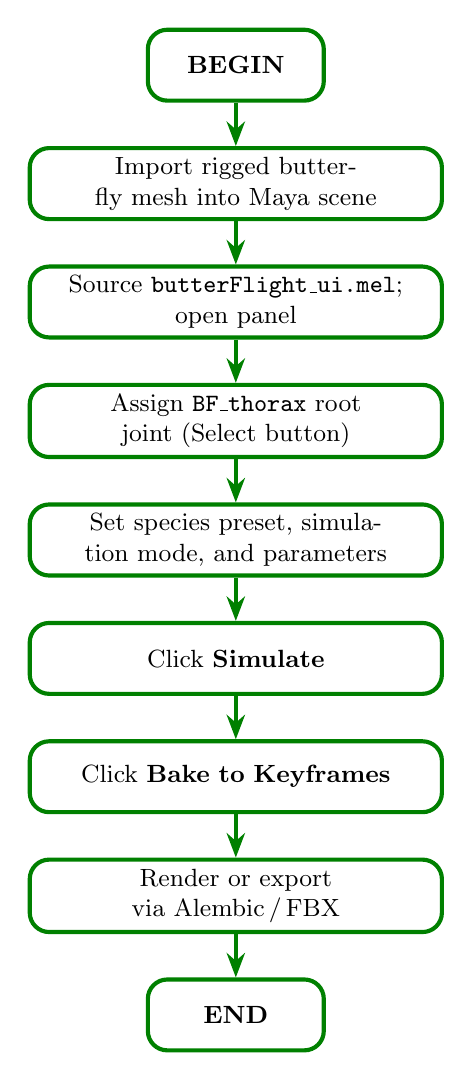
\begin{tikzpicture}[
    node distance=0.55cm,
    proc/.style={
        rectangle, rounded corners=7pt,
        draw=green!50!black, line width=1.5pt,
        text centered, text width=5.0cm,
        minimum height=0.9cm, fill=white, font=\small},
    startstop/.style={
        rectangle, rounded corners=7pt,
        draw=green!50!black, line width=1.5pt,
        text centered, text width=2.0cm,
        minimum height=0.9cm, fill=white,
        font=\small\bfseries},
    dec/.style={
        diamond, aspect=2.6,
        draw=green!50!black, line width=1.5pt,
        text centered, text width=2.8cm,
        inner sep=2pt, fill=white, font=\small},
    arr/.style={->, >=Stealth, line width=1.3pt, color=green!50!black}]

\node[startstop]                    (begin)   {BEGIN};
\node[proc, below=of begin]         (import)  {Import rigged butterfly mesh into Maya scene};
\node[proc, below=of import]        (open)    {Source \texttt{butterFlight\_ui.mel}; open panel};
\node[proc, below=of open]          (assign)  {Assign \texttt{BF\_thorax} root joint (Select button)};
\node[proc, below=of assign]        (params)  {Set species preset, simulation mode, and parameters};
\node[proc, below=of params]        (simulate){Click \textbf{Simulate}};
\node[proc, below=of simulate]      (bake)    {Click \textbf{Bake to Keyframes}};
\node[proc, below=of bake]          (export)  {Render or export via Alembic\,/\,FBX};
\node[startstop, below=of export]   (end)     {END};

% Main vertical flow
\draw[arr] (begin)   -- (import);
\draw[arr] (import)  -- (open);
\draw[arr] (open)    -- (assign);
\draw[arr] (assign)  -- (params);
\draw[arr] (params)  -- (simulate);
\draw[arr] (simulate)-- (bake);
\draw[arr] (bake)    -- (export);
\draw[arr] (export)  -- (end);

\end{tikzpicture}
\caption{ButterFlight workflow. After opening the panel and assigning a rig, the user
  configures species, mode, and simulation parameters, runs the simulation, then
  bakes the result to standard Maya keyframes and optionally triggers an Alembic or
  FBX export.}
\label{fig:workflow}
\end{figure}


\newpage

% ========== Section 2: Authoring Tool Development ==========
\section{Authoring Tool Development}

\subsection{Technical Approach}

\subsubsection{Algorithm Details}

The simulation is organized into three inter-connected modules that mirror
the structure of Chen et al.\ 2022.

% ---------- Module 1 ----------
\textbf{Module 1: Butterfly Modeling (paper Section~4).}

The butterfly body is represented by a hierarchical skeleton of nine joints.
The \textbf{thorax} is the root and has one degree of freedom (DOF): pitch angle
$\theta_\beta$. Each \textbf{fore-wing} (left and right) has three DOFs:
flap angle $\theta_\gamma$, feather angle $\theta_\zeta$, and sweep angle
$\theta_\psi$. Each \textbf{hind-wing} has one DOF: flap angle $\theta_\gamma$
only, because its aerodynamic contribution is secondary and its motion closely
tracks the fore-wings. The \textbf{abdomen} has one DOF: rotation $\theta_\phi$
along the body longitudinal axis. In total the model has five independently
parameterized angles, collected as
$\chi = \{\theta_\beta, \theta_\gamma, \theta_\zeta, \theta_\psi, \theta_\phi\}$.

All five maneuvering angles are computed via the \textbf{maneuvering function}
(Equation~1 of the paper):
\[
  \theta^{*}\!\bigl(\varphi_a^{*}(\mathbf{u}),\,f^{*}(\mathbf{u}),\,
  \varphi_p^{*},\,\varphi_m^{*},\,t\bigr)
  \;=\;
  \varphi_a^{*}(\mathbf{u})\cos\!\bigl(2\pi f^{*}(\mathbf{u})\,t
  + \varphi_p^{*}\bigr) + \varphi_m^{*},
  \quad * \in \{\beta,\gamma,\zeta,\psi,\phi\}
\]
where $\mathbf{u}$ is the current butterfly velocity, $\varphi_a^{*}$ is the
amplitude, $f^{*}$ is the frequency, $\varphi_p^{*}$ is the phase offset, and
$\varphi_m^{*}$ is the mean angle. Both $f^{*}$ and $\varphi_a^{*}$ are
sigmoid functions of speed (Equations~2--3):
\[
  f^{*}\!\bigl(\mathbf{u}(t_0)\bigr)
  = \frac{R_f^{*}}{1 + e^{-16\,(\,|\mathbf{u}(t_0)|/|\mathbf{u}_{\max}| - 0.5\,)}},
  \qquad
  \varphi_a^{*}\!\bigl(\mathbf{u}(t_0)\bigr)
  = \frac{R_{\theta_a}^{*}}{1 + e^{-16\,(\,|\mathbf{u}(t_0)|/|\mathbf{u}_{\max}| - 0.5\,)}}
\]
so that both frequency and amplitude increase smoothly with speed. The phase
offsets $\varphi_p^{*}$ are $0^\circ$ for the fore-wing and hind-wing flap angles,
$-180^\circ$ for the abdomen (to reproduce the counterphase oscillation observed
in real Monarch butterflies~\cite{Sridhar2016}), and $-90^\circ$ for the thorax.
Frequency and amplitude are held constant within one flapping cycle
($t_0 \to t_1$) and updated at each cycle boundary using a sliding-window smoother
(Module~3 below). The parameter ranges used in our implementation are taken
directly from Table~3 of the paper and are listed in Table~\ref{tab:params}.

\begin{table}[H]
\centering\small
\begin{tabular}{|l|c|c|c|c|}
\hline
\textbf{Angle} & $R_f^{*}$ (Hz) & $R_{\theta_a}^{*}$ ($^\circ$)
               & $\varphi_p^{*}$ ($^\circ$) & $\varphi_m^{*}$ ($^\circ$) \\
\hline
$\theta_\beta$  & $0$--$3$   & $0$--$30$  & $-90$  & $0$   \\
$\theta_\gamma$ & $0$--$11$  & $0$--$150$ & $0$    & $10$  \\
$\theta_\zeta$  & $0$--$11$  & $0$--$10$  & $-90$  & $0$   \\
$\theta_\psi$   & $0$--$11$  & $0$--$20$  & $-90$    & $0$   \\
$\theta_\phi$   & $0$--$11$   & $0$--$35$  & $-180$ & $-10$ \\
\hline
\end{tabular}
\caption{Maneuvering angle parameter ranges from Chen et al.\ 2022, Table~3.}
\label{tab:params}
\end{table}

% ---------- Module 2 ----------
\textbf{Module 2: Forces Computation (paper Section~5).}

Two forces act on the butterfly at each time step.

\textit{(a) Simplified Aerodynamic Force (Section~5.1).}
Following the quasi-steady theory of Ellington~(1984a)~\cite{Ellington1984a},
the lift and drag forces on the $i$-th polygon of wing $j$ are:
\[
  \mathbf{F}_{i,\mathrm{lift}} = \tfrac{1}{2}\rho A_i |\mathbf{V}|^2 C_l(\alpha),
  \qquad
  \mathbf{F}_{i,\mathrm{drag}} = \tfrac{1}{2}\rho A_i |\mathbf{V}|^2 C_d(\alpha),
\]
where $\rho$ is air density, $A_i$ is the polygon area, and $\mathbf{V}$ is the
air velocity over the wing surface. The local angle of attack is
$\alpha = \arctan(|\mathbf{V}_n|/|\mathbf{V}_t|)$,
with $\mathbf{V}_n$ the normal component and $\mathbf{V}_t$ the tangential
(base-to-tip) component. The empirical lift and drag coefficient polynomials
proposed by the paper are:
\[
  C_l(\alpha) = -0.0095953\alpha^2 + 0.090635\alpha - 0.34182,
\]
\[
  C_d(\alpha) = -0.0000079518\alpha^3 + 0.0011527\alpha^2 + 0.0063148\alpha + 0.51127.
\]
The total aerodynamic force on wing $j$ is the polygon sum
$\mathbf{F}_j = \sum_i \mathbf{F}_{i,j}$, and all four wings contribute
to the resultant $\sum_{j=1}^{4}\mathbf{F}_j$.

\textit{(b) Curl-Noise Vortex Force (Section~5.2).}
To reproduce the inherently chaotic, vortex-driven trajectory noise of real
butterfly flight, a vortex force is computed from a curl-noise field
(Bridson et al.\ 2007~\cite{Bridson2007}) seeded with Perlin noise
(Perlin 2002~\cite{Perlin2002}):
\[
  \mathbf{F}_{\mathrm{vor}}
  = \nabla \times
    \Bigl(\tfrac{s_1(\mathbf{p})}{\textit{gain}_x},\;
          \tfrac{s_2(\mathbf{p})}{\textit{gain}_y},\;
          \tfrac{s_3(\mathbf{p})}{\textit{gain}_z}\Bigr)\cdot\eta,
\]
where $\mathbf{p}$ is the center of mass of the thorax, $s_1, s_2, s_3$ are
Perlin noise values at $\mathbf{p}$ with different seeds, and $\eta$ scales the
force magnitude. The paper sets $\textit{gain}_x = \textit{gain}_z = 22.0$,
$\textit{gain}_y = 5.5$, and $\eta = 3.66$ empirically. Smaller gain values
produce tighter vortices; larger values produce broader, gentler noise. Crucially,
$\mathbf{F}_{\mathrm{vor}}$ is applied \emph{only} to the thorax center of mass,
not to individual wing polygons, to avoid excessive uncontrolled wing twisting.

% ---------- Module 3 ----------
\textbf{Module 3: Maneuvering Control (paper Section~6).}

Body translation and posture are decoupled. Velocity is computed from the
composite of all forces acting on the butterfly, while posture angles are updated
separately via the maneuvering functions above.

\textit{(a) Velocity Computation (Section~6.1).}
If the butterfly is targeting a point $\mathbf{q}_i$ (path keypoint or
attraction target), a preferred acceleration is computed from a vision-based
ramp function:
\[
  \mathbf{a}_{\mathrm{pre}} = \frac{R(d)}{m}\cdot\frac{\mathbf{p}-\mathbf{q}_i}{|\mathbf{p}-\mathbf{q}_i|},
  \qquad
  d = \min\!\Bigl(1,\,\frac{|\mathbf{p}-\mathbf{q}_i|}{L}\Bigr),
\]
where $m$ is the butterfly mass and $L = 4.5$ is the field-of-view sensing
length. The local acceleration from the force model is:
\[
  \mathbf{a}_{\mathrm{loc}}
  = \Bigl(\sum_{j=1}^{4}\mathbf{F}_j + \mathbf{F}_{\mathrm{vor}} + \mathbf{g}\Bigr)\big/m,
\]
and the velocity at time step $t$ is updated as:
\[
  \mathbf{u}_t = \mathbf{u}_{t-1} + (\mathbf{a}_{\mathrm{loc}} + \mathbf{a}_{\mathrm{pre}})\,\Delta t.
\]

\textit{(b) Maneuvering Update (Section~6.2).}
Between flapping cycles, both frequency $f^*$ and amplitude $\varphi_a^*$ are
smoothed by a sliding-window average to prevent abrupt transitions:
\[
  c^*_{n+1}
  = 0.5\!\sum_{i=\max(n-k,1)}^{n-1} w_i\,c^*_i \;+\; 0.5\,c^*_n,
  \quad * \in \{f, \varphi_a\},\quad \sum w_i = 1,
\]
where $c^*_n$ is the parameter value at flapping cycle $n$ (computed from
Equations~2--3), and $k = 10$ is the sliding window size.

% ---------- Assumptions ----------
\textbf{Assumptions and Simplifications.}

\begin{itemize}
  \item \textbf{Synchronous bilateral wings.} Left and right wings (fore and hind)
    are assumed to flap with the same frequency and amplitude at all times.
    This is consistent with biological observations for normal forward flight
    but precludes banked turning simulation.

  \item \textbf{Fixed parameters within one flapping cycle.} Both $f^*$ and
    $\varphi_a^*$ are held constant from $t_0$ to $t_1$ and only updated at
    cycle boundaries. This simplifies the integration and avoids intra-cycle
    discontinuities, at the cost of slightly reduced responsiveness to
    instantaneous velocity changes.

  \item \textbf{Quasi-steady aerodynamics.} We use the quasi-steady thin-wing
    approximation rather than a full Navier-Stokes/CFD solver. This is orders
    of magnitude faster but ignores leading-edge vortex dynamics and
    unsteady wake interactions between wing strokes.

  \item \textbf{Empirical polynomial coefficients.} The lift and drag coefficient
    curves $C_l(\alpha)$ and $C_d(\alpha)$ are fitted from experimental data
    and applied uniformly across both species. Species-specific coefficients
    are not available in the paper and are not modeled.

  \item \textbf{Vortex force at thorax CoM only.} Applying $\mathbf{F}_{\mathrm{vor}}$
    to the thorax rather than individual wing polygons avoids uncontrolled twisting.
    The vortex force therefore influences body trajectory and through-velocity
    also affects wing frequency and amplitude, but does not directly drive
    wing deformation.

  \item \textbf{Maya joint system instead of Unity Dynamic Bone.} The paper's
    original implementation uses Unity's Dynamic Bone component for skeleton
    spring deformation. In ButterFlight we replicate the kinematic joint angles
    via direct \texttt{setAttr} and \texttt{setKeyframe} calls on Maya joints;
    no spring physics are applied to the skeleton itself.

  \item \textbf{No takeoff or landing.} The simulation assumes the butterfly is
    always in steady forward or hovering flight. Takeoff momentum from leg jumping
    and landing coordination are outside the scope of this implementation.
\end{itemize}

\subsubsection{Maya Interface and Integration}

ButterFlight is split across two implementation layers: a \textbf{MEL scripting layer}
responsible for all user-facing interaction, and a \textbf{C++ plug-in layer}
(\texttt{butterFlight.mll}) that performs the computationally intensive simulation and
keyframe writing. The two layers communicate through a single Maya command registered
by the plug-in.

\textbf{MEL / Python layer} (\texttt{butterFlight\_ui.mel}).
All GUI elements are created with standard MEL UI commands
(\texttt{window}, \texttt{frameLayout}, \texttt{columnLayout},
\texttt{optionMenuGrp}, \texttt{floatFieldGrp}, \texttt{button}, etc.).
The MEL layer has no simulation logic; its only responsibilities are:
\begin{itemize}
  \item Constructing and displaying the panel window.
  \item Validating user inputs (joint prefix check, empty-field guards).
  \item Collecting parameter values from all controls and forwarding them
        as flags to the C++ command \texttt{butterFlightSimulate}.
  \item Calling \texttt{bakeResults} on the rig hierarchy after simulation,
        and optionally invoking \texttt{AbcExport} or the FBX plug-in for export.
  \item Providing the \textit{Reset} function that restores all control defaults.
\end{itemize}
Scene-setup utilities (e.g., checking that the required \texttt{BF\_} joints exist,
querying NURBS curve CVs for path keypoints) may be implemented in Python using the
\texttt{maya.cmds} API for easier string handling.

\textbf{C++ plug-in layer} (\texttt{butterFlight.mll}).
The plug-in is built as a Maya API plug-in using the Maya 2026 C++ SDK and registered
via the standard \texttt{MFnPlugin} mechanism. It exposes one custom
\texttt{MPxCommand} subclass:

\begin{itemize}
  \item \textbf{\texttt{BFSimulateCmd} (subclass of \texttt{MPxCommand})}.
    Parses all simulation flags (rig root, mode, species parameters, force
    parameters, frame range), runs the per-frame simulation loop, and writes
    joint rotations and root translations directly to the scene using
    \texttt{MFnAnimCurve} and \texttt{MAnimControl}.
    The command is undoable: it caches the pre-existing animation curves and
    restores them in its \texttt{undoIt()} method.
\end{itemize}

The key Maya API classes used by the plug-in are summarised below:

\begin{table}[H]
\centering\small
\begin{tabular}{|l|l|}
\hline
\textbf{Maya API class} & \textbf{Role in ButterFlight} \\
\hline
\texttt{MPxCommand}       & Base class for \texttt{BFSimulateCmd}; provides undo support \\
\texttt{MFnDagNode}       & Traverses the joint hierarchy from \texttt{BF\_thorax} \\
\texttt{MFnIkJoint}       & Reads and sets joint rotation attributes ($\theta_\beta$, $\theta_\gamma$, etc.) \\
\texttt{MFnTransform}     & Sets world-space root translation at each simulated frame \\
\texttt{MFnAnimCurve}     & Creates and writes \texttt{animCurveTA/TL} nodes for baked output \\
\texttt{MFnNurbsCurve}    & Samples CVs of the user-specified path curve for Path Following mode \\
\texttt{MAnimControl}     & Queries current frame rate and time unit for $\Delta t$ computation \\
\texttt{MVector / MPoint} & Stores velocity $\mathbf{u}$, position $\mathbf{p}$, and force vectors \\
\texttt{MArgDatabase}     & Parses command-line flags passed from the MEL layer \\
\hline
\end{tabular}
\caption{Maya API classes used by \texttt{butterFlight.mll}.}
\label{tab:api}
\end{table}

The simulation loop inside \texttt{BFSimulateCmd::doIt()} iterates over every
frame in the requested range. At each frame it: (1)~evaluates the five maneuvering
angles using Module~1 equations; (2)~computes per-polygon aerodynamic forces by
querying wing mesh normals via \texttt{MFnMesh}; (3)~evaluates the curl-noise
vortex force at the thorax CoM; (4)~integrates velocity via Newton's second law;
(5)~updates joint rotations and root position; and (6)~writes one keyframe per
joint via \texttt{MFnAnimCurve::addKey}.

\subsubsection{Software Design and Development}

ButterFlight follows a three-tier architecture that separates user-facing controls,
simulation logic, and Maya scene manipulation into distinct layers
(Figure~\ref{fig:arch}).

\begin{figure}[H]
\centering
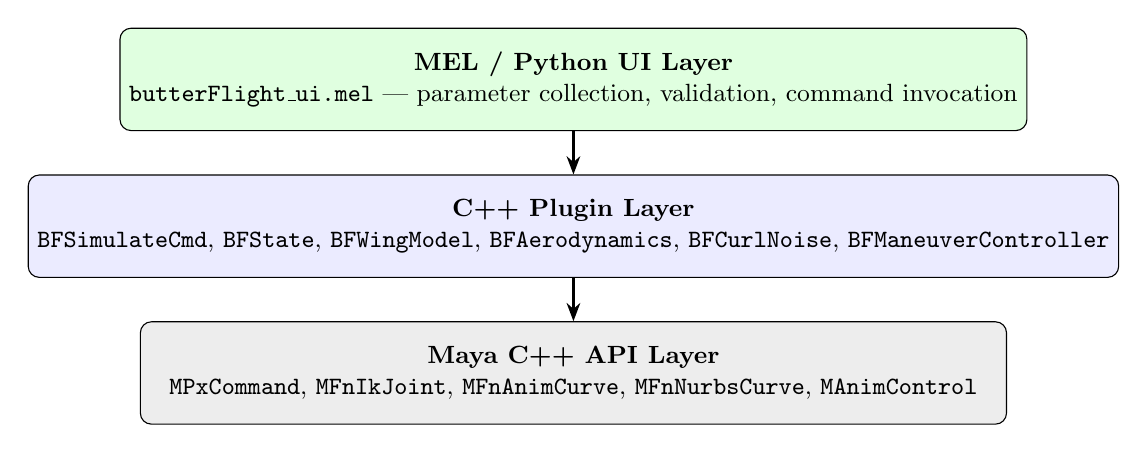
\begin{tikzpicture}[
  box/.style={draw, rounded corners=4pt, minimum width=11cm, minimum height=1.3cm,
              align=center, font=\small},
  arr/.style={-Stealth, thick}]
  \node[box, fill=green!12] (mel)
    {\textbf{MEL / Python UI Layer}\\
     \texttt{butterFlight\_ui.mel} --- parameter collection, validation,
     command invocation};
  \node[box, fill=blue!8, below=0.55cm of mel] (cpp)
    {\textbf{C++ Plugin Layer}\\
     \texttt{BFSimulateCmd}, \texttt{BFState}, \texttt{BFWingModel},
     \texttt{BFAerodynamics}, \texttt{BFCurlNoise}, \texttt{BFManeuverController}};
  \node[box, fill=gray!14, below=0.55cm of cpp] (api)
    {\textbf{Maya C++ API Layer}\\
     \texttt{MPxCommand}, \texttt{MFnIkJoint}, \texttt{MFnAnimCurve},
     \texttt{MFnNurbsCurve}, \texttt{MAnimControl}};
  \draw[arr] (mel) -- (cpp);
  \draw[arr] (cpp) -- (api);
\end{tikzpicture}
\caption{ButterFlight three-tier software architecture.}
\label{fig:arch}
\end{figure}

\paragraph{Class hierarchy.}
The C++ plugin layer is organized around six classes:

\begin{itemize}
  \item \textbf{BFSimulateCmd} (\texttt{MPxCommand} subclass) --- Entry point
    registered with Maya as the \texttt{bfSimulate} command. Parses
    \texttt{MArgDatabase} flags, orchestrates the per-frame simulation loop,
    and implements \texttt{undoIt}/\texttt{redoIt} by caching original keyframe
    data before any curves are written.

  \item \textbf{BFState} (plain struct) --- Per-butterfly value aggregate: world-space
    position (\texttt{MPoint}), velocity (\texttt{MVector}), the nine joint-angle
    values $\theta^*$, phase accumulator $t$, and a circular buffer of the last
    $k=10$ control-point positions used by the sliding-window smoother.

  \item \textbf{BFWingModel} --- Evaluates Equations~1--3 each frame to compute
    target joint angles given the current maneuvering inputs. Stores
    species-specific parameters: mass, wing area, nominal flapping frequency,
    amplitude, and phase offsets for each joint.

  \item \textbf{BFAerodynamics} --- Computes quasi-steady lift and drag forces
    (Equations~4--6) for each of the four wings using the angle of attack between
    the wing-panel normal and the local velocity vector relative to the surrounding
    air.

  \item \textbf{BFCurlNoise} --- Generates the curl of a 3-D Perlin noise field
    (Equation~7) at a query position using a finite-difference curl approximation.
    Applies the species-independent gain and $\eta$ constants to produce the vortex
    force applied to the thorax centre of mass.

  \item \textbf{BFManeuverController} --- Implements the preferred-acceleration and
    local-acceleration decoupling (Equations~8--11) and the sliding-window smoother
    (Equation~12) that drives the body trajectory along a path or swarm target.
\end{itemize}

\paragraph{Key data flow.}
\texttt{BFSimulateCmd::doIt} initialises a \texttt{BFState} at the start frame,
then iterates frame by frame. Each iteration calls \texttt{BFWingModel::update}
$\to$ \texttt{BFAerodynamics::computeForces} $\to$ \texttt{BFCurlNoise::eval}
$\to$ \texttt{BFManeuverController::step}, accumulates the resulting net
acceleration into \texttt{BFState::velocity} and \texttt{position}, and finally
writes joint rotations and root position to Maya animation curves via
\texttt{MFnAnimCurve::addKey}.

\paragraph{Third-party dependencies.}
\begin{itemize}
  \item \textbf{Maya 2026 C++ devkit} (Autodesk, included with Maya 2026) ---
    provides all \texttt{MFn*} and \texttt{MPx*} headers and import libraries.
  \item \textbf{No additional runtime libraries} --- all vector and matrix arithmetic
    is performed with Maya's built-in \texttt{MVector}, \texttt{MPoint}, and
    \texttt{MMatrix} types; no external linear-algebra library (e.g., Eigen) is
    required.
  \item \textbf{CMake 3.25+} (build system only) --- used to locate the Maya devkit
    and generate the Visual Studio solution; not required at runtime.
\end{itemize}

\subsection{Target Platforms}

\subsubsection{Hardware}

Table~\ref{tab:hw} lists the minimum and recommended hardware configurations
for running ButterFlight inside Autodesk Maya 2026 on Windows.

\begin{table}[H]
\centering
\caption{Hardware requirements.}
\label{tab:hw}
\begin{tabular}{|l|p{4.8cm}|p{4.8cm}|}
\hline
\textbf{Component} & \textbf{Minimum} & \textbf{Recommended} \\
\hline
Processor &
  Intel Core i5 (8th gen) or AMD Ryzen 5 3600, 2.5\,GHz+, 4 cores &
  Intel Core i7/i9 or AMD Ryzen 7/9, 3.0\,GHz+, 8+ cores \\
\hline
RAM & 8\,GB & 16\,GB or more \\
\hline
GPU &
  Any GPU supported by Maya 2026 Viewport 2.0 &
  NVIDIA RTX or AMD RDNA GPU with 4\,GB+ VRAM \\
\hline
Storage & 10\,GB free disk space & SSD with 20\,GB free \\
\hline
Display & 1920$\times$1080 & 2560$\times$1440 or higher \\
\hline
\end{tabular}
\end{table}

The ButterFlight simulation itself is a CPU-bound, single-threaded computation;
no GPU is used by the plug-in directly. However, Maya's Viewport 2.0 renderer
leverages the GPU for scene display, so a capable GPU meaningfully reduces total
iteration time when previewing animations.

\subsubsection{Software}

Table~\ref{tab:sw} lists all required and optional software for building and
running ButterFlight.

\begin{table}[H]
\centering
\caption{Software requirements.}
\label{tab:sw}
\begin{tabular}{|l|l|p{4.5cm}|}
\hline
\textbf{Software} & \textbf{Required Version} & \textbf{Notes} \\
\hline
Operating System &
  Windows 10 64-bit (v1903+) or Windows 11 &
  No macOS or Linux support at this time \\
\hline
Autodesk Maya &
  Maya 2026 &
  Plug-in compiled against the Maya 2026 devkit \\
\hline
C++ Compiler &
  Visual Studio 2022 (v17.x), MSVC 14.3+ &
  Desktop Development with C++ workload required \\
\hline
Windows SDK &
  10.0.19041.0 or later &
  Included in the VS 2022 installer \\
\hline
Maya devkit &
  Maya 2026 Developer Kit &
  Required to build the \texttt{.mll} plug-in \\
\hline
Build system &
  CMake 3.25 or later &
  Generates the Visual Studio solution; build-time only \\
\hline
VC++ Redistributable &
  Microsoft VC++ 2022 Redistributable (x64) &
  Bundled with Maya 2026; not needed separately \\
\hline
FBX plug-in &
  Bundled with Maya 2026 &
  For keyframe animation export \\
\hline
Alembic I/O plug-in &
  Bundled with Maya 2026 &
  Optional; for point-cache export \\
\hline
\end{tabular}
\end{table}

ButterFlight is compiled as a Maya plug-in (\texttt{.mll}) targeting Maya 2026
on Windows. The MEL script layer (\texttt{butterFlight\_ui.mel}) runs inside
Maya's embedded MEL interpreter and requires no separate Python or scripting-runtime
installation. All build instructions assume Visual Studio 2022 with the Desktop
Development with C++ workload; CMake locates the Maya devkit headers and generates
the Visual Studio project automatically.

\subsection{Software Versions}

\subsubsection{Alpha Version Features (first prototype)}

The alpha release establishes the core single-butterfly simulation pipeline with
path-following locomotion. It targets the milestone date of \textbf{March 25}.

\paragraph{Included features.}
\begin{itemize}
  \item \textbf{Single butterfly, path-follow mode} --- the user selects a NURBS
    curve as the flight path; the butterfly's thorax centre of mass tracks the
    curve while maneuvering control (Module 3) handles orientation and speed.
  \item \textbf{Default species model (Monarch preset)} --- fixed mass $0.428\,$g,
    wing area $26\,$cm$^2$, and nominal flapping parameters; no custom-species
    input in this version.
  \item \textbf{Full wing kinematics (Module 1)} --- all nine joints animated per
    frame using the maneuvering function (Eq.~1) with sigmoid frequency and
    amplitude (Eqs.~2--3).
  \item \textbf{Quasi-steady aerodynamics (Module 2)} --- lift and drag computed
    each frame from wing-panel normals and local velocity; curl-noise vortex force
    applied to the thorax to produce natural trajectory noise.
  \item \textbf{Bake to Keyframes} --- simulation output written to Maya animation
    curves on the rig joints, playable without the plug-in loaded.
  \item \textbf{Basic MEL UI panel} --- Rig Assignment, Path Settings, Force
    Parameters, and Output Settings sections; Simulate and Bake to Keys buttons.
\end{itemize}

\paragraph{Alpha demo scene.}
The alpha demo consists of a rigged Monarch butterfly mesh and a gently curving
NURBS path placed above a flat ground plane. Running \textit{Simulate} produces
roughly 200 frames of path-following flight with visible wing-abdomen coupling and
aerodynamic trajectory noise. The scene ships as \texttt{scenes/alpha\_demo.mb}
and requires only the \texttt{.mll} plug-in and \texttt{butterFlight\_ui.mel} to
reproduce.

\subsubsection{Beta Version Features}

The beta release extends the alpha with wind simulation, swarm locomotion, and
custom species support. It targets the milestone date of \textbf{April 15} and
delivers a feature-complete tool ahead of the final demo.

\paragraph{New features added upon alpha.}
\begin{itemize}
  \item \textbf{Wind (curl-noise vortex)} --- a Wind section in the UI exposes
    per-axis gain and the $\eta$ scale factor; enabling wind applies
    \texttt{BFCurlNoise} forces each frame, producing visibly erratic, turbulent
    trajectories that vary between simulation runs.
  \item \textbf{Swarm mode} --- the user specifies a butterfly count (2--20) and
    an aggregation centre point; each butterfly receives its own \texttt{BFState}
    and an individual preferred-acceleration target derived from the swarm
    centroid, producing loosely coordinated flock behaviour.
%   \item \textbf{Custom species parameters} --- selecting the \textit{Custom} preset
%     in the Species section unlocks all mass, wing-area, frequency, and amplitude
%     fields so artists can dial in non-standard insects or stylised creatures.
%   \item \textbf{Swallowtail preset} --- a second built-in preset ($0.34\,$g,
%     $28\,$cm$^2$) auto-fills species parameters for Papilio butterfly proportions.
  \item \textbf{Alembic / FBX export integration} --- the Bake to Keys step is
    complemented by an \textit{Export Cache} button that fires Maya's built-in
    Alembic or FBX export after baking, writing a self-contained cache file.
  \item \textbf{Full MEL UI panel} --- the Species Preset, Wind, and Swarm Settings
    sections (hidden in alpha) become active; mode-switching between Path and Swarm
    dynamically shows or hides the relevant control groups.
\end{itemize}

\paragraph{Beta demo scene.}
The beta demo provides two scenes:
\begin{enumerate}
  \item \texttt{scenes/beta\_wind\_demo.mb} --- a single Monarch on a curved path
    with wind enabled; the trajectory deviates noticeably from the path at moderate
    gain values, illustrating the vortex-force contribution.
  \item \texttt{scenes/beta\_swarm\_demo.mb} --- five Monarchs initialised at
    random offsets around a shared aggregation point, simulated for 300 frames to
    show loose cohesion and individual wing-motion variation.
\end{enumerate}

\subsubsection{Description of Demos and Tutorials}

The final release ships with three ready-to-open Maya scene files and an
in-panel \textit{Quick-Start} guide, all located in the \texttt{scenes/} and
\texttt{doc/} directories of the repository.

\paragraph{Demo scenes.}
\begin{itemize}
  \item \textbf{Alpha path-follow demo} (\texttt{scenes/alpha\_demo.mb}) ---
    a Monarch butterfly following a curved NURBS path; demonstrates baseline wing
    kinematics, abdomen coupling, and quasi-steady aerodynamic noise with no wind.
    Intended as the simplest entry point for first-time users.

  \item \textbf{Wind turbulence demo} (\texttt{scenes/beta\_wind\_demo.mb}) ---
    the same path scene with wind enabled at moderate gain values. Highlights how
    curl-noise vortex forces perturb the trajectory while the maneuvering controller
    continues to track the path. Useful for comparing wind-on versus wind-off output.

  \item \textbf{Swarm demo} (\texttt{scenes/beta\_swarm\_demo.mb}) ---
    five Monarchs aggregating around a shared centroid point over 300 frames.
    Demonstrates per-agent \texttt{BFState} independence, loose cohesion, and
    natural variation in individual flapping phase.
\end{itemize}

\paragraph{Quick-Start tutorial.}
A \textit{Quick-Start} PDF (\texttt{doc/QuickStart.pdf}) walks a new user through
the complete workflow in ten annotated steps, mirroring the Work Flow described in
Section~1.4.3.

\newpage

% ========== Section 3: Work Plan ==========
\section{Work Plan}

\subsection{Tasks and Subtasks}

\noindent\textbf{Task 1 --- Environment Setup and Maya Plugin Scaffolding}\\
\textbf{Duration:} 1 week \quad \textbf{Assigned:} Cecilia Chen, Yiding Tian

This task establishes the build environment and the minimal plugin skeleton required
by all subsequent tasks. It covers configuring CMake to locate the Maya 2026 devkit,
producing a loadable \texttt{.mll} file, and verifying the MEL-to-C++ command
round-trip. Completing this task unblocks parallel development of the simulation
modules.

\begin{itemize}
  \item \textbf{Subtask 1.1 --- CMake Build Configuration}: Configure
    \texttt{CMakeLists.txt} to locate the Maya 2026 devkit headers and import
    libraries, generate a Visual Studio 2022 solution, and produce a signed
    \texttt{butterFlight.mll} that loads cleanly in Maya's Plug-in Manager.
  \item \textbf{Subtask 1.2 --- BFSimulateCmd Skeleton}: Implement and register a
    minimal \texttt{BFSimulateCmd} (MPxCommand subclass) that accepts a
    \texttt{-startFrame}/\texttt{-endFrame} flag pair and prints a confirmation
    string to the Script Editor without performing any simulation.
  \item \textbf{Subtask 1.3 --- MEL Round-Trip Verification}: Write the opening
    \texttt{butterFlight\_ui.mel} stub (window with a single Simulate button) and
    confirm that clicking it successfully invokes \texttt{bfSimulate} and reads the
    Script Editor output, proving the full MEL-to-C++ pipeline is functional.
\end{itemize}

\bigskip
\noindent\textbf{Task 2 --- Butterfly Skeleton Rig and Maneuvering Functions}\\
\textbf{Duration:} 2 weeks \quad \textbf{Assigned:} Yiding Tian

This task implements \texttt{BFWingModel} and the \texttt{BFState} data structure,
which together form the kinematic backbone of the simulation. The maneuvering
function (Eq.~1) and its sigmoid modifiers (Eqs.~2--3) must produce visually
plausible wing motion for the Monarch preset before aerodynamic forces are added.
Correct joint-rotation application via \texttt{MFnIkJoint} and \texttt{MFnTransform}
is verified by scrubbing the timeline manually.

\begin{itemize}
  \item \textbf{Subtask 2.1 --- BFState Struct and Joint Enum}: Define the
    \texttt{BFState} plain-old-data struct (position, velocity, nine joint angles,
    phase accumulator, sliding-window circular buffer) and a \texttt{BFJoint} enum
    mapping the nine skeleton joints to array indices.
  \item \textbf{Subtask 2.2 --- Maneuvering Function (Eqs.~1--3)}: Implement
    \texttt{BFWingModel::update}, which computes target joint angles $\theta^*$ each
    frame using the cosine maneuvering function and the sigmoid frequency and
    amplitude modifiers, seeded with the species-specific nominal values from
    Table~\ref{tab:params}.
  \item \textbf{Subtask 2.3 --- Joint-Rotation Applicator}: Write the helper that
    retrieves each named joint (\texttt{BF\_thorax}, \texttt{BF\_forewing\_L}, etc.)
    via \texttt{MFnDagNode} and sets its local rotation via \texttt{MFnTransform},
    enforcing the correct rotation order (XYZ) to match the paper's DOF conventions.
  \item \textbf{Subtask 2.4 --- Visual Verification}: Manually scrub a 60-frame
    preview with the Monarch preset and confirm that forewing flap, feather, and
    sweep joints animate correctly, the hindwings follow in phase, and the abdomen
    rotates counter-phase to the thorax pitch.
\end{itemize}

\bigskip
\noindent\textbf{Task 3 --- Aerodynamic Force Model}\\
\textbf{Duration:} 1.5 weeks \quad \textbf{Assigned:} Cecilia Chen

This task implements \texttt{BFAerodynamics}, which computes per-wing quasi-steady
lift and drag forces (Eqs.~4--6) each frame using the empirical polynomial
coefficients from the paper. Wing-panel normals are derived from the joint world
transforms rather than mesh face normals, avoiding a costly mesh query. The
resulting forces are accumulated into \texttt{BFState::velocity} via Newton's second
law and the per-frame timestep.

\begin{itemize}
  \item \textbf{Subtask 3.1 --- Wing-Panel Normal Computation}: Approximate each
    wing panel's outward normal from the cross product of the forewing joint's local
    X and Y axes in world space, providing the geometric input needed for
    angle-of-attack computation without querying \texttt{MFnMesh}.
  \item \textbf{Subtask 3.2 --- Lift/Drag Polynomial Evaluation (Eqs.~4--6)}:
    Implement the $C_l(\alpha)$ and $C_d(\alpha)$ empirical polynomial evaluators
    and the lift/drag force equations using air density $\rho=1.225\,\text{kg/m}^3$
    and per-wing panel area from \texttt{BFWingModel}.
  \item \textbf{Subtask 3.3 --- Newton Integration}: Accumulate net aerodynamic
    force across all four wings, divide by butterfly mass to obtain acceleration,
    and add it to \texttt{BFState::velocity} scaled by the per-frame timestep
    $\Delta t = 1/\text{fps}$.
\end{itemize}

\bigskip
\noindent\textbf{Task 4 --- Curl-Noise Vortex Force}\\
\textbf{Duration:} 1 week \quad \textbf{Assigned:} Cecilia Chen

This task implements \texttt{BFCurlNoise}, which generates turbulent vortex forces
(Eq.~7) at the thorax centre of mass by taking the curl of a three-dimensional
Perlin gradient noise field. The finite-difference curl approximation avoids the
closed-form derivative, keeping the implementation straightforward. Gain constants
(\textit{gain\_x} $=$ \textit{gain\_z} $= 22.0$, \textit{gain\_y} $= 5.5$,
$\eta = 3.66$) are hardcoded as defaults and exposed through the MEL UI Wind section.

\begin{itemize}
  \item \textbf{Subtask 4.1 --- 3-D Gradient Perlin Noise}: Implement a
    gradient-based Perlin noise function suitable for three-dimensional queries,
    using a permutation table and quintic interpolation to match the smoothness
    properties required by the curl approximation.
  \item \textbf{Subtask 4.2 --- Finite-Difference Curl (Eq.~7)}: Compute
    $\nabla \times (s_1/g_x,\, s_2/g_y,\, s_3/g_z)$ via forward finite differences
    with step size $\epsilon = 0.01$, then scale by $\eta$ to produce the vortex
    force vector applied to the thorax.
  \item \textbf{Subtask 4.3 --- UI Integration}: Wire the Wind section of the MEL
    panel (\textit{Enable Wind} checkbox and gain sliders) to flags on
    \texttt{bfSimulate}, and verify that toggling wind on and off produces
    noticeably different trajectory noise in a 100-frame test run.
\end{itemize}

\bigskip
\noindent\textbf{Task 5 --- Maneuvering Control and Body Motion Decoupling}\\
\textbf{Duration:} 1.5 weeks \quad \textbf{Assigned:} Yiding Tian

This task implements \texttt{BFManeuverController}, which decouples body locomotion
from wing kinematics by computing a preferred acceleration toward the path or swarm
target and a local aerodynamic correction (Eqs.~8--12). The sliding-window smoother
($k=10$) is stored in the circular buffer inside \texttt{BFState} and is updated
each frame before joint angles are applied. Correct path-following behaviour at this
stage is the primary acceptance criterion for the alpha milestone.

\begin{itemize}
  \item \textbf{Subtask 5.1 --- Preferred Acceleration (Eq.~8)}: Implement the
    ramp function that computes preferred acceleration toward the next path CV or
    swarm centroid, clamped by the species maximum speed, and blended with a look-ahead
    distance to prevent overshooting sharp curves.
  \item \textbf{Subtask 5.2 --- Local Acceleration Decoupling (Eqs.~10--11)}:
    Compute local aerodynamic acceleration from the net wing forces and subtract
    the component already accounted for by preferred acceleration, then integrate
    both into \texttt{BFState::velocity} and \texttt{position} per Eq.~11.
  \item \textbf{Subtask 5.3 --- Sliding-Window Smoother (Eq.~12)}: Implement the
    $k=10$ weighted circular buffer in \texttt{BFState} and apply the smoother to
    the body control-point position each frame, verifying that the resulting
    trajectory is smooth relative to a raw (unsmoothened) reference run.
\end{itemize}

\bigskip
\noindent\textbf{Task 6 --- MEL/Python UI Panel}\\
\textbf{Duration:} 1 week \quad \textbf{Assigned:} Cecilia Chen

This task completes \texttt{butterFlight\_ui.mel} with all eight collapsible
frameLayout sections, species-preset auto-fill, mode-dependent section visibility,
and the three action buttons. The panel must correctly collect every parameter and
forward it as a flag to the \texttt{bfSimulate} command, and the Bake to Keys button
must invoke Maya's \texttt{bakeResults} on the correct joint set. This task also
includes usability testing to ensure the panel behaves correctly on first load.

\begin{itemize}
  \item \textbf{Subtask 6.1 --- Full Control Layout}: Implement all eight
    frameLayout sections (Rig Assignment, Species Preset, Simulation Mode, Path
    Settings, Wind, Force Parameters, Swarm Settings, Output Settings) with correct
    control types, default values, and collapsible state.
  \item \textbf{Subtask 6.2 --- Callbacks}: Implement \texttt{bfUpdateMode}
    (show/hide Path and Swarm sections), \texttt{bfUpdateSpecies} (auto-fill and
    lock fields for named presets, unlock for Custom), and \texttt{bfWindToggle}
    (enable/disable gain sliders).
  \item \textbf{Subtask 6.3 --- Command Invocation and Bake}: Implement
    \texttt{bfSimulate} (collect all control values and call the C++ command with
    assembled flags) and \texttt{bfBakeKeyframes} (query the rig root, enumerate
    descendant joints, and call \texttt{bakeResults} over the simulation frame
    range).
\end{itemize}

\bigskip
\noindent\textbf{Task 7 --- Single Butterfly Path-Following Demo (Alpha)}\\
\textbf{Duration:} 0.5 weeks \quad \textbf{Assigned:} Cecilia Chen, Yiding Tian

This integration task assembles Tasks 1--6 into a working alpha build and creates
the \texttt{alpha\_demo.mb} scene. Any joint-rotation-order bugs, world-space
transform errors, or flag-passing mismatches between MEL and C++ that appear during
end-to-end testing are resolved here. Completion of this task marks the
\textbf{Alpha milestone (March 25)}.

\begin{itemize}
  \item \textbf{Subtask 7.1 --- End-to-End Integration Test}: Load the plugin and
    MEL panel, assign a rigged Monarch mesh to a NURBS path, run Simulate for
    200 frames, and confirm that joint animation curves are written correctly to the
    rig without Maya errors or crashes.
  \item \textbf{Subtask 7.2 --- Integration Bug Fixes}: Resolve any discrepancies
    between expected and observed joint motion (rotation-order mismatches, incorrect
    world-to-local transforms, frame-offset errors) identified during Subtask 7.1.
  \item \textbf{Subtask 7.3 --- Alpha Scene Packaging}: Save the verified scene as
    \texttt{scenes/alpha\_demo.mb}, document the required plugin and MEL file in the
    README, and tag the Git repository at the alpha commit.
\end{itemize}

\bigskip
\noindent\textbf{Task 8 --- Swarm Simulation and Aggregation}\\
\textbf{Duration:} 1.5 weeks \quad \textbf{Assigned:} Yiding Tian

This task extends \texttt{BFSimulateCmd} to manage multiple independent
\texttt{BFState} instances and computes per-agent preferred acceleration offsets
toward the evolving swarm centroid. Each butterfly in the swarm runs the full
Module~1--3 pipeline independently, so wing-motion variation arises naturally from
different initial phase accumulators. The swarm count (2--20) and the aggregation
target transform are exposed through the Swarm Settings section of the MEL UI.

\begin{itemize}
  \item \textbf{Subtask 8.1 --- Multi-Agent State Management}: Extend
    \texttt{BFSimulateCmd::doIt} to accept a \texttt{-count} flag, allocate a
    \texttt{BFState} vector of length $N$, and initialise each agent at a random
    position within a user-specified radius of the aggregation target.
  \item \textbf{Subtask 8.2 --- Centroid-Based Preferred Acceleration}: Each frame,
    compute the current swarm centroid from all agent positions and inject it as the
    preferred-acceleration target for every agent via
    \texttt{BFManeuverController::step}, producing loose cohesion without explicit
    collision avoidance.
  \item \textbf{Subtask 8.3 --- Swarm UI and Demo Scene}: Wire the butterfly count
    spinner and aggregation-target picker in the Swarm Settings section, add a
    \texttt{-swarmTarget} flag to \texttt{bfSimulate}, and create
    \texttt{scenes/beta\_swarm\_demo.mb} with five Monarchs for the beta milestone.
\end{itemize}

\bigskip
\noindent\textbf{Task 9 --- Export, Wind Polish, and Beta Integration}\\
\textbf{Duration:} 0.5 weeks \quad \textbf{Assigned:} Cecilia Chen

This task completes the beta feature set by adding the Alembic/FBX Export Cache
button, finalising wind parameter round-tripping, and creating the
\texttt{beta\_wind\_demo.mb} scene. It also includes a final UI polish pass
(tooltip text, error messages for missing rig, and graceful handling of an empty
path selection). Completion of this task marks the \textbf{Beta milestone
(April 15)}.

\begin{itemize}
  \item \textbf{Subtask 9.1 --- Export Cache Button}: Add an \textit{Export Cache}
    button to the Output Settings section that first calls \texttt{bfBakeKeyframes}
    and then invokes Maya's \texttt{AbcExport} or \texttt{FBXExport} command on the
    rig hierarchy, writing a timestamped cache file to the project's
    \texttt{cache/} directory.
  \item \textbf{Subtask 9.2 --- Wind Parameter Round-Trip}: Verify that all Wind
    gain and $\eta$ values entered in the MEL UI are correctly forwarded as
    \texttt{bfSimulate} flags, stored in \texttt{BFCurlNoise}, and produce
    reproducible output when the same seed is used across runs.
  \item \textbf{Subtask 9.3 --- Beta Scene Packaging and Tag}: Save
    \texttt{scenes/beta\_wind\_demo.mb} demonstrating visible trajectory deviation
    under moderate wind, verify both beta demo scenes play back without the plugin
    loaded (baked curves only), and tag the Git repository at the beta commit.
\end{itemize}

\bigskip
\noindent\textbf{Task 10 --- Testing, Debugging, and Final Demo Scenes}\\
\textbf{Duration:} 1 week \quad \textbf{Assigned:} Cecilia Chen, Yiding Tian

The final task validates all three demo scenes against expected behaviour, profiles
swarm performance for $N=20$ butterflies, and produces the Quick-Start PDF and any
remaining documentation. Any bugs surfaced by full-scene regression testing are
triaged and fixed here. Completion of this task satisfies the \textbf{Final Demo
(May 5)} and \textbf{Code Submission (May 11)} milestones.

\begin{itemize}
  \item \textbf{Subtask 10.1 --- Regression Testing}: Run all three demo scenes
    from a clean Maya session (plugin loaded fresh, no cached state) and verify
    that wing motion, trajectory noise, and baked curves match the expected output
    documented in Section~2.3.
  \item \textbf{Subtask 10.2 --- Swarm Performance Profiling}: Simulate a
    $N=20$ swarm for 300 frames and record per-frame compute time; if any frame
    exceeds 2 seconds on the recommended hardware configuration, profile the inner
    loop and apply targeted optimisations (e.g., precomputed normals, SIMD noise
    evaluation).
  \item \textbf{Subtask 10.3 --- Quick-Start PDF and Code Submission}: Write the
    ten-step Quick-Start tutorial with annotated screenshots, export it as
    \texttt{doc/QuickStart.pdf}, verify the repository README includes build and
    load instructions, and submit the final codebase by May 11.
\end{itemize}

\subsection{Milestones}

\subsubsection{Alpha Version}

\textbf{Target date: March 25.} \quad
The alpha milestone delivers a single-butterfly, path-following simulation with
full wing kinematics and aerodynamic forces. The following tasks and subtasks must
be complete:

\begin{itemize}
  \item \textbf{Task 1 (all subtasks)} --- Build system configured, \texttt{.mll}
    loads in Maya's Plug-in Manager, and MEL-to-C++ round-trip verified.
  \item \textbf{Task 2 (all subtasks)} --- \texttt{BFState} struct defined;
    \texttt{BFWingModel::update} animates all nine joints correctly for the Monarch
    preset; visual verification passed.
  \item \textbf{Task 3 (all subtasks)} --- \texttt{BFAerodynamics} computes per-wing
    lift and drag each frame; Newton integration accumulates forces into velocity.
  \item \textbf{Task 4, Subtasks 4.1--4.2} --- \texttt{BFCurlNoise} generates
    vortex force at the thorax CoM with correct gain and $\eta$ constants. (UI
    exposure, Subtask 4.3, may be deferred to beta if time is tight.)
  \item \textbf{Task 5 (all subtasks)} --- \texttt{BFManeuverController} implements
    preferred and local acceleration decoupling; sliding-window smoother ($k=10$)
    produces a smooth path-following trajectory.
  \item \textbf{Task 6 (all subtasks)} --- MEL panel with Rig Assignment, Path
    Settings, Force Parameters, and Output Settings sections; Simulate, Bake to Keys,
    and Reset buttons all functional.
  \item \textbf{Task 7 (all subtasks)} --- End-to-end integration test passed;
    \texttt{scenes/alpha\_demo.mb} created and Git repository tagged at the alpha
    commit.
\end{itemize}

\noindent\textbf{Acceptance criteria.}
An evaluator opening \texttt{scenes/alpha\_demo.mb}, loading the plugin and MEL
panel, clicking \textit{Simulate}, and then \textit{Bake to Keyframes} should
see: (1)~a Monarch butterfly tracking a curved NURBS path for 200 frames;
(2)~all nine joints animated with visible wing-abdomen counter-phase coupling;
(3)~mild aerodynamic trajectory noise even in the absence of wind; and
(4)~fully baked animation curves on the rig joints that play back without the
plugin loaded.

\subsubsection{Beta Version}

\textbf{Target date: April 15.} \quad
The beta milestone extends the alpha with wind simulation, swarm locomotion,
custom species support, and export. All alpha tasks remain complete; the following
additional tasks must also be finished:

\begin{itemize}
  \item \textbf{Task 4, Subtask 4.3} --- Wind section in the MEL panel wired to
    \texttt{BFCurlNoise}; enable/disable toggle and per-axis gain sliders functional.
  \item \textbf{Task 6 (beta UI additions)} --- Swarm Settings section visible when Swarm
    mode is selected; Wind section active.
  \item \textbf{Task 8 (all subtasks)} --- Multi-agent \texttt{BFState} management
    in \texttt{BFSimulateCmd}; centroid-based preferred acceleration for swarm
    cohesion; Swarm Settings UI wired; 
    \\ \texttt{scenes/beta\_swarm\_demo.mb} created.
  \item \textbf{Task 9 (all subtasks)} --- Export Cache button invokes Alembic or
    FBX export after baking; wind parameter round-trip verified;
    \texttt{scenes/beta\_wind\_demo.mb} created; Git repository tagged at the beta
    commit.
\end{itemize}

\noindent\textbf{Acceptance criteria.}
In addition to all alpha criteria, an evaluator should be able to: (1)~enable Wind
and observe visibly erratic trajectory deviation from the NURBS path in \\
\texttt{scenes/beta\_wind\_demo.mb}; (2)~open \texttt{scenes/beta\_swarm\_demo.mb},
run Simulate with five butterflies, and see loosely cohesive swarm behaviour with
per-agent wing-motion variation; (3)~click \textit{Export Cache} and receive a
valid \texttt{.abc} or \texttt{.fbx} file; and (4)~select the Swallowtail preset
and observe different mass and wing-area values auto-filled in the panel.

\subsection{Schedule}

% TODO: Insert Gantt chart showing all tasks, durations, and milestone dates
% (alpha: Mar 25, beta: Apr 15, final demo: May 5, code due: May 11).

% Placeholder for Gantt chart:
% \begin{figure}[H]
%   \centering
%   \includegraphics[width=\textwidth]{figures/gantt.png}
%   \caption{ButterFlight project schedule}
% \end{figure}

\newpage

% ========== Section 4: Related Research ==========
\section{Related Research}

% The Related Research section is fulfilled by including the Literature Survey.
% Insert the content of Literature_Survey_ButterFlight.tex here,
% or \input it directly:
%
% \input{../Literature_Survey/Literature_Survey_ButterFlight_content.tex}

% TODO: Paste or \input the full Literature Survey content (introduction,
% research evolution graph, paper descriptions, and references).

\newpage

% ========== Bibliography ==========
\begin{thebibliography}{99}

\bibitem{Chen2022}
CHEN Q., LU T., TONG Y., LUO G., JIN X., DENG Z.:
A Practical Model for Realistic Butterfly Flight Simulation.
\textit{ACM Transactions on Graphics (TOG)} 1, 1 (2022), 12 pages.

\bibitem{Ellington1984a}
ELLINGTON C.~P.:
The aerodynamics of hovering insect flight. I. The quasi-steady analysis.
\textit{Philosophical Transactions of the Royal Society of London. B,
Biological Sciences} 305, 1122 (1984), 1--15.

\bibitem{Ellington1984b}
ELLINGTON C.~P.:
The aerodynamics of hovering insect flight. V. A vortex theory.
\textit{Philosophical Transactions of the Royal Society of London. B,
Biological Sciences} 305, 1122 (1984), 115--144.

\bibitem{Reynolds1987}
REYNOLDS C.~W.:
Flocks, herds and schools: A distributed behavioral model.
In \textit{Proceedings of the 14th Annual Conference on Computer Graphics
and Interactive Techniques} (1987), pp.~25--34.

\bibitem{BettsWootton1988}
BETTS C.~R., WOOTTON R.~J.:
Wing shape and flight behaviour in butterflies (Lepidoptera: Papilionoidea
and Hesperioidea): a preliminary analysis.
\textit{Journal of Experimental Biology} 138, 1 (1988), 271--288.

\bibitem{Perlin2002}
PERLIN K.:
Improving noise.
In \textit{ACM Transactions on Graphics (TOG)}, Vol.~21.
ACM, 2002, pp.~681--682.

\bibitem{WuPopovic2003}
WU J., POPOVI\'C Z.:
Realistic modeling of bird flight animations.
\textit{ACM Transactions on Graphics (TOG)} 22, 3 (2003), 888--895.

\bibitem{Bridson2007}
BRIDSON R., HOURIHAM J., NORDENSTAM M.:
Curl-noise for procedural fluid flow.
\textit{ACM Transactions on Graphics (TOG)} 26, 3 (2007), 46--es.

\bibitem{WilsonAlbertani2014}
WILSON T., ALBERTANI R.:
Wing-flapping and abdomen actuation optimization for hovering in the
butterfly \textit{Idea leuconoe}.
In \textit{52nd Aerospace Sciences Meeting} (2014), 0009.

\bibitem{Wang2014}
WANG X., JIN X., DENG Z., ZHOU L.:
Inherent noise-aware insect swarm simulation.
In \textit{Computer Graphics Forum}, Vol.~33.
Wiley Online Library, 2014, pp.~51--62.

\bibitem{Wang2015}
WANG X., REN J., JIN X., MANOCHA D.:
BSwarm: biologically-plausible dynamics model of insect swarms.
\textit{Proceedings of the 14th ACM SIGGRAPH/Eurographics Symposium on
Computer Animation} (2015), 111--118.

\bibitem{Sridhar2016}
SRIDHAR M., KANG C.-K., LANDRUM D.~B.:
Instantaneous lift and motion characteristics of butterflies in free flight.
In \textit{46th AIAA Fluid Dynamics Conference} (2016), 3252.

\bibitem{Chen2019}
CHEN Q., LUO G., TONG Y., JIN X., DENG Z.:
Shape-constrained flying insects animation.
\textit{Computer Animation and Virtual Worlds} 30, 3--4 (2019), e1902.

\bibitem{Sridhar2020}
SRIDHAR M., KANG C.-K., LEE T.:
Geometric formulation for the dynamics of monarch butterfly with the effects
of abdomen undulation.
In \textit{AIAA Scitech 2020 Forum} (2020), 1962.

\bibitem{Will2020}
WILL H.:
Dynamic Bone.
Unity Asset Store, 2020.
\url{https://assetstore.unity.com/packages/tools/animation/dynamic-bone-16743}.

\end{thebibliography}

\end{document}
